\section{Úvod}

Význam distribuovaných algoritmov v súčasnosti narastá, a spolu s ním narastá aj potreba
zahrnúť distribuované algoritmy do výučby. Myslíme si, že by sa táto téma dala oveľa lepšie naučiť
z prehľadnej vizualizácie, než z kníh a zložito písaných textov.

Rozhodli sme sa teda vytvoriť aplikáciu, ktorá by ľuďom interaktívnym a čo najlepším spôsobom
vysvetľovala fungovanie mnohých distribuovaných algoritmov, a ktorá by mu pomohla prehĺbiť a lepšie si zapamätať
novonadobudnuté znalosti. Myslíme si totiž, že v tejto oblasti existuje mnoho pekných úvah a trikov,
ktoré je dobré si osvojiť. 

Ďalší prvok, ktorým by sme chceli pomôcť vo výučbe a spoznávaní týchto algoritmov, je umožnenie užívateľovi, 
aby si sám vyskúšal naprogramovať niektoré z nich a zároveň by užívateľ mal byť schopný sám
ovplyvňovať dianie algoritmov. Toto by malo preklenúť medzeru medzi porozumením a schopnosťou
aplikácie.

Medzi algoritmy, ktoré sme zatiaľ zvizualizovali, patrí distribuované prehľadávanie do šírky,
taktiež voľba šéfa na úplnom grafe a traverzovanie. Okrem toho, že plánujeme pridať nové 
algoritmy, je užívateľ schopný sám vytvoriť algoritmus, ktorý mu naša aplikácia zvizualizuje.

Zvyšok článku je organizovaný nasledovne: v sekcii $2$ si povieme, v akom výpočtovom modeli
pracujeme a fungujú spomínané tri distribuované algoritmy. 
Následne v sekcii $3$ popíšeme samotnú implementáciu aplikácie, ako
funguje a prečo sme veci robili tak, ako sme ich robili. Nakoniec v sekcii $4$ spomenieme naše plány do budúcnosti.

\noindent
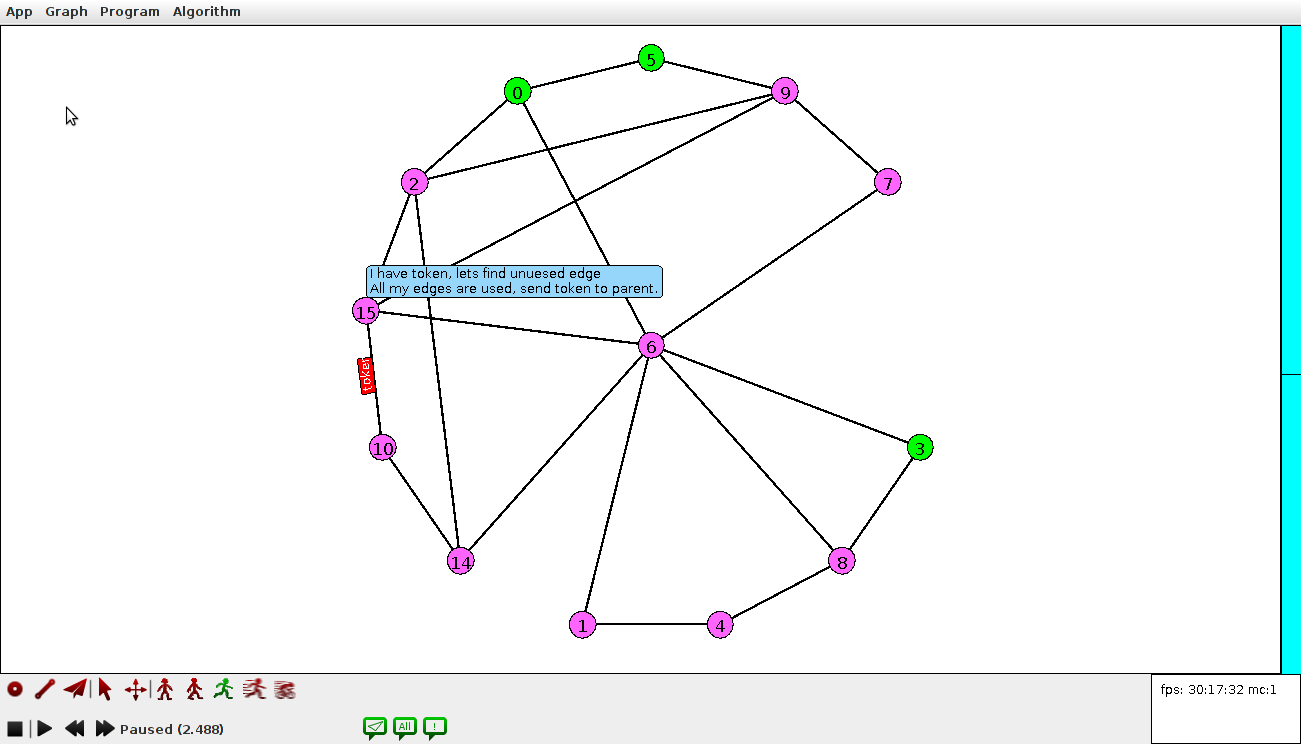
\includegraphics[width=8.5cm]{DFS.png}